\documentclass[%
tikz,
convert={outfile=\jobname.png},
preview=true,
multi=false,
varwidth=true,
border=8px,
]
{standalone}

\usepackage{amsmath}

\begin{document}
 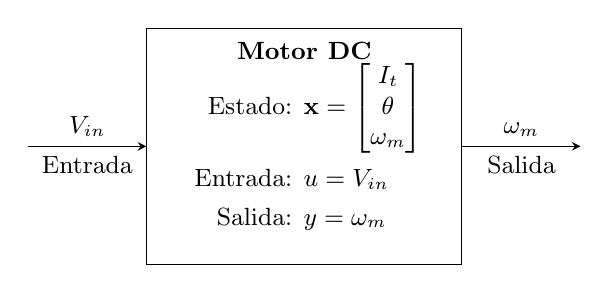
\begin{tikzpicture}[
      >=stealth,
      block/.style={draw, rectangle, minimum width=4cm, minimum height=3cm, align=center},
      every node/.style={font=\small}
    ]
    
    % Caja negra principal
    \node[block] (system) at (0,0) {
      \textbf{Motor DC} \\
      \vspace{0.2cm}
      $\begin{aligned}
        \text{Estado: } & \mathbf{x} = 
        \begin{bmatrix}
          I_t \\ \theta \\ \omega_m
        \end{bmatrix} \\
        \text{Entrada: } & u = V_{in} \\
        \text{Salida: } & y = \omega_m
      \end{aligned}$
    };
    
    % Entrada
    \draw[<-] (system.west) -- ++(-1.5,0) 
      node[midway, above] {$V_{in}$}
      node[midway, below] {Entrada};
    
    % Salida
    \draw[->] (system.east) -- ++(1.5,0) 
      node[midway, above] {$\omega_m$}
      node[midway, below] {Salida};
    
  \end{tikzpicture}
 \end{document}
